\begin{frame}[fragile]{Tutorial: n-site states with MPS}

\begin{columns}

\begin{column}{6cm}

\begin{onlyenv}<1->
\begin{lstlisting}[language=JuliaLocal, style=julia, mathescape, basicstyle=\scriptsize\ttfamily]
  j = n ÷ 2
  Xj = op("X", i[j])

  XjZp = apply(Xj, Zp);


  st = [k == j ? "Zm" : "Zp"
        for k in 1:n];
  XjZp = MPS(i, st);
\end{lstlisting}
\end{onlyenv}

\begin{onlyenv}<3->
\begin{lstlisting}[language=JuliaLocal, style=julia, mathescape, basicstyle=\scriptsize\ttfamily]
  maxlinkdim(XjZp) == 1
  inner(Zp, XjZp) == 0
\end{lstlisting}
\end{onlyenv}

\end{column}

\begin{column}{4.5cm}

\begin{onlyenv}<1-1>
~\\
~\\
~\\
$X_j|Z+Z+\dots Z+\rangle =$ \\
$|Z+Z+\dots Z-\dots Z+\rangle$ \\
~\\
~\\
$|Z+Z+\dots Z-\dots Z+\rangle$ \\
~\\
\end{onlyenv}

\begin{onlyenv}<2->
\vspace*{0.0cm}
\begin{center}
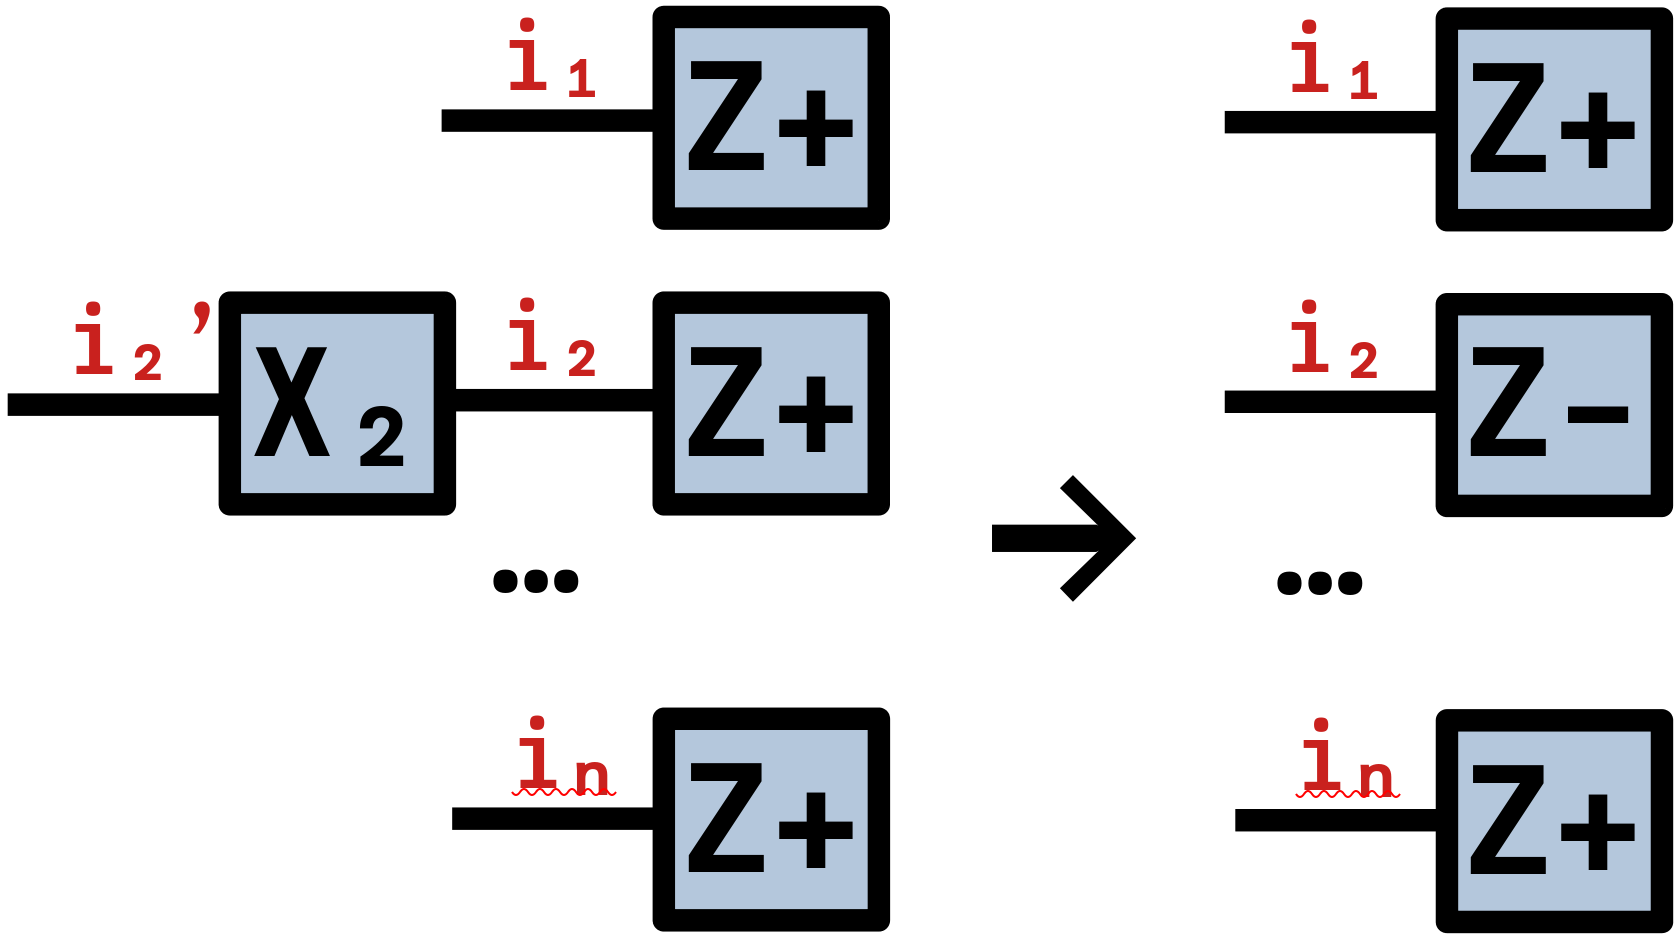
\includegraphics[width=1.0\textwidth]{
  slides/assets/XjZpn.png
}
\end{center}
\vspace*{0.0cm}
\end{onlyenv}

\begin{onlyenv}<3->
~\\
~\\
~\\
~\\
~\\
\end{onlyenv}

\end{column}

\end{columns}

\end{frame}
